\section{Core Person Registration Process}
\label{core_person_registration_process}

The figure \ref{fig:person_registration_flow} is an activity diagram that shows visually the flow of the registration of a \textbf{Person}. As evidenced by \cite{alfedaghi2021validationconceptualversusactivity}, a UML activity diagram is a semi-formal semantic specification that is intuitive and flexible. It is used to describe a system's behaviors and the internal logic of complex operations. Therefore, it is widely utilized as a front-end tool for the system-level design of software and hardware systems. 

\begin{figure}[HContext]
    \centering
    \caption{Flow of the Registration of a Person}
    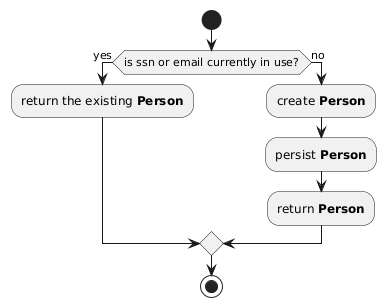
\includegraphics[width=1\linewidthContext]
    {figures/person_registration_activity_diagram.png}
    \label{fig:person_registration_flow}
    \footnotesize Source: Author's creation.
\end{figure}

If the verification discovers that the provided SSN or email is already associated with a persisted \textbf{Person}, it is retrieved. Otherwise, a new instance of \textbf{Person} is created and persisted.